\subsection{redundancy coding}
	\begin{frame}{source coding}{redundancy coding 1/2}
		\begin{figure}
			\centering
				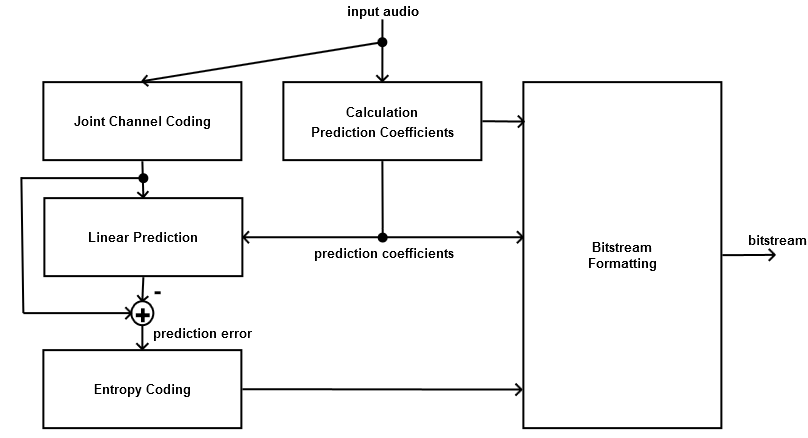
\includegraphics[scale=0.4]{Graph/redundancycoding}
		\end{figure}
	\end{frame}

	\begin{frame}{source coding}{redundancy coding 2/2}	
		\begin{itemize}
			\item	\textbf{properties}
				\begin{itemize}
					\item	perfect signal reconstruction
					\item	bitrate reduction depends on input signal
						\begin{itemize}
							\item	typical gain (stereo, 48k): factor 2
						\end{itemize}
					\item	no constant bitrate $\rightarrow$ streaming only with large buffers
				\end{itemize}
			\pause
            \bigskip
			\item	\textbf{common applications/algorithms}
			\begin{table}
			\centering
				\begin{footnotesize}
					\begin{tabular}{lccc}
					\hline
						\textbf{name} & \textbf{sampling rates}	& \textbf{channels}	& \textbf{word length} \\
					\hline
					Shorten	& all 			& 2 	& 8/16\\
					FLAC 	& 1-1048k 		& 8 	& 4-32\\
					MLP 	& 44.1k-192k	& 63 	& 1-24\\
					ALS 	& all 			& 65536	& 1-32 (int), 32(float)\\
					\end{tabular}  
				\end{footnotesize}
			\end{table}
		\end{itemize}		
	\end{frame}
